\section{Mini-projet d'e-banking}

À la suite de notre formation, nous avons mis en pratique nos connaissances dans un mini-projet de réalisation d'une application web d'e-banking.

\subsection{Cahier des charges}

L'application à réaliser est une application web de gestion des comptes. Les fonctionnalités sont les suivantes :

\begin{itemize}
	\item S'identifier,
	\item Consulter la liste de ses comptes,
	\item Consulter le détail des opérations pour un compte et un mois donné,
	\item Consulter le détail des opérations cartes pour un compte et un mois donné,
	\item Effectuer un virement entre ses comptes,
	\item Consulter l'historique de ses virements,
	\item Exporter au format Excel le relevé des opérations pour un mois donné.
	\item Exposer ces fonctionnalités sous la forme de web services.
\end{itemize}

\subsection{Gestion du projet}

Étant cinq stagiaires à être arrivés le même jour et un autre la semaine suivante, nous avons formé une équipe de six personnes pour réaliser ce projet. Il nous avait été laissé la possibilité de former deux groupes projet de trois personnes, mais nous avons préférer former une seule équipe et ainsi avoir la possibilité d'approfondir de façon plus importante le projet.\\

La méthode que nous avons utilisé pour gérer ce projet a été un mélange entre la méthode Scrum et l'XP, soit deux méthodes Agiles. L'utilisation des méthodes Agiles repose en grande partie sur le constat qu'un produit logiciel voit la plupart du temps ses demandes en fonctionnalités évoluer au fur et à mesure, et que cela est très difficile à prendre en compte avec un  système non itératif, comme pas exemple le cycle en V. Ici, le but est d'effectuer de courtes itérations d'une à deux semaines au bout desquelles un produit utilisable est livré. Dans notre cas, du fait de la durée du projet, nous avons fait des itérations (ou sprints) d'une semaine.\\

La première itération, appelé Sprint 0 a consisté en la mise en place de l'environnement de développement, de l'environnement d'intégration ainsi que des conventions à utiliser. C'est au cours de cette semaine que nous avons aussi choisi le socle de technologies que nous utiliserions. Nous avons aussi réfléchi à l'architecture générale de l'application. Tous ces choix sont expliqué dans la suite du rapport. À la fin de ce premier Sprint, nous avons fait une réunion avec Stéphane LANDELLE, le directeur technique d'\ebi{}, pour valider nos choix.\\

Les autres itérations ce sont ensuite déroulées de la façon suivante :
\begin{enumerate}
	\item Réunion avec le \flqq{}product owner\frqq{} (client dans le vocabulaire Scrum), c'est à dire Stéphane LANDELLE, pour sélectionner les fonctionnalités à développer dans cette itération,
	
	\item Développement des fonctionnalités, principalement en pair programming pour mutualiser les connaissances,
	
	\item Réunion technique avec Stéphane LANDELLE en tant que référent technique pour auditer notre code,
	
	\item Remaniement (refactoring) du code suite aux remarques.
	
	\item Réunion avec le \flqq{}product owner\frqq{} pour présenter les fonctionnalités implémentées.\\
\end{enumerate}

De plus, chaque jour nous réalisions un \flqq{}daily Scrum\frqq{} à heure fixe : c'est une courte réunion dans laquelle tout les intervenants sont debout, pour pousser à la concision, et répondent à trois questions :
\begin{enumerate}
	\item Qu'est-ce que j'ai fait hier ?
	
	\item Qu'est-ce que je compte faire aujourd'hui ?
	
	\item Quelles sont les difficultés que je rencontre ?\\
\end{enumerate}

Cette méthode permet d'avoir un résultat chaque semaine à montrer au client. Le client peut donc voir l'évolution du projet en temps réel, tester les parties déjà développées ce qui permet d'avoir un retour rapide. De plus, le client est beaucoup plus investi dans le projet et peut facilement ajuster ou modifier le cahier des charges.\\

Pour le développeur, les itérations permettent de ne pas avoir un travail trop répétitif puisque dans chaque itération, on retrouve toutes les phases du cycle en V classique. Il n'y a donc plus de grandes phases de développement, de tests, de recette, \dots{}

\subsection{Choix techniques}

Le choix des technologies à utiliser était en grande partie libre, même s'il était soumis à l'approbation de Stéphane. Voici les technologies que nous avons choisi :

\subsubsection{Gestionnaire de version}

Il permet de travailler sur un projet de manière collaborative et simultanée. Il existe principalement deux gestionnaires de version : Git et Subversion, dont la philosophie diffère.\\

Subversion est le plus répandu actuellement car plus ancien. C'est un système de versionnement centralisé, i.e. qu'il n'existe qu'un seul dépôt des versions, robuste qui à fait ses preuves. Le développement est fortement linéaire, car la création d'une branche demande la copie complète du code.

Git est lui plus récent (2005). Il a été créé par Linus Torvalds pour gérer le développement du noyaux Linux. C'est un système de versionnement décentralisé, chaque utilisateur dispose d'un dépôt local, très puissant. Il tire profit au maximum des branches pour avoir des fonctionnalités se développant en parallèle sans rentrer en conflit. Une fois une fonctionnalité développée sa branche est fusionnée à la branche principale généralement appelée master.\\

Nous avons choisi d'utiliser Git, car même si ce n'est pas actuellement le système le plus utilisé, la puissance et la flexibilité qu'il apporte en feront surement le leader dans un futur proche. De plus l'utilisation de cette outil nous a permis de mettre en place un processus d'intégration continue très intéressant qui sera détaillé ci-après. Malgré son coté décentralisé nous avions besoin d'un dépôt distant permettant de centraliser le travail et d'accéder au code de n'importe où. Nous avons ainsi choisi d'héberger notre projet sur GitHub, plateforme d'hébergement de projet open-source utilisant Git. 

\subsubsection{Construction du projet}

Plusieurs systèmes permettent de construire des projets Ant, Maven, Gradle, \dots{} Ant est le plus ancien. C'est globalement un outil qui permet d'écrire des scripts pour construire des applications. Il est très apprécié car il est très flexible.\\

Maven est plus récent, s'appuie sur des script de build en XML, et se base sur le principe de \flqq{}convention over configuration\frqq{}, c'est à dire qu'il encourage le développeur à respecter certaines conventions pour faciliter la construction du projet comme par exemple l'arborescence du projet, i.e. emplacement des sources, des sources de test \dots{}. Il inclut aussi un système de gestion de dépendance qui va directement chercher les librairies externes dans des dépôts Maven accessibles publiquement.\\

Gradle quant à lui est le plus récent. Il reprend beaucoup des principes de Maven, notamment la gestion des dépendances et le principe de \flqq{}convention over configuration\frqq{}, mais permet aussi une plus grande flexibilité se rapprochant ainsi plus de Ant, grâce à des script écrit en Groovy.\\

Nous avons choisi Maven car c'est actuellement le plus utilisé en entreprise et qu'il est pour des projets relativement classique le plus abouti.

\subsubsection{Système de Gestion de Base de Données (SGBD)}

Afin de persister nos données nous avons besoin d'un SGBD. Il existe de nombreuses possibilités et l'application à réaliser n'a pas besoin de fonctionnalités avancées hormis une gestion des transactions pour garantir la cohérence de nos tables.\\

Les deux principaux SGBD open source sont MySQL et PostgreSQL. Ces deux solutions sont assez proches. Nous avons choisi PostgreSQL pour son plus grand respect de la norme SQL.

\subsubsection{ORM}

Le choix de d'Hibernate comme ORM nous a été imposé. En effet il est actuellement le standard de facto et sa maitrise est un impératif de notre métier. Nous avons par contre choisi d'utiliser la version 4, qui est une implémentation de la spécification JPA. Il est a noter que l'implémentation de référence de cette spécification est TopLink, mais qu'elle est beaucoup moins utilisée. 

\subsubsection{Conteneur d'application}

Les conteneurs d'applications sont des boites à outils fournissant des services pour résoudre des problématiques que toute application rencontre. Dans le monde Java, il en existe principalement deux : JEE et Spring.\\

A nouveau le choix de Spring nous a été imposé. Car même si il n'est pas porté par un standard Spring est le conteneur le plus répandu dans le monde de l'entreprise. Spring est un conteneur léger qui ne nécessite pas un serveur d'application mais un simple conteneur de Servlet contrairement au conteneur JEE. Ceci permet d'éviter, au moins pour le développement de l'application, la complexité, la lenteur et la lourdeur de serveur comme JBoss, Weblogic ou Websphere et de simplement déployer son application dans un Tomcat ou un Jetty qui sont beaucoup plus rapide.\\

De plus, nous avons aussi utiliser Spring pour l'intégration d'Hibernate (Spring-DB), la gestion des transactions (Spring-TX), le framework MVC (Spring-MVC), la sécurité (Spring-Security) et la mise en place de traitement batch (Spring-Batch). 

\subsubsection{Serveur}

Puisque nous utilisons Spring, nous pouvons utiliser un simple conteneur de Servlet. Il en existe principalement deux Jetty et Apache Tomcat. Nous avons préféré Tomcat car encore une fois, il est le plus répandu et que sa robustesse n'est plus a démontrer. Il sert entre autre de conteneur de Servlet dans le serveur JBoss et sert par exemple en production chez Atos Worldline. 

\subsubsection{Frameworks de tests}

Les tests sont une composante importante d'un projet informatique. Il existe différents types de tests qui répondent à différentes problématique.

Tout d'abord les tests unitaires qui vont permettre de s'assurer du bon fonctionnement et de la non régression d'un composant logiciel. Dans ce but nous avons utilisé JUnit, qui est le standard de facto dans le monde Java. D'autre alternative existe comme TestNG qui d'un point de vue strictement technique est plus performant. Mais la prédominance de JUnit dans le monde professionnel nous a fait préférer cette solution.\\

Pour pouvoir isoler les composants logiciel lors des tests unitaires nous avons aussi utilisé un framework de mock. Mocker un objet consiste à remplacer un objet par un faux dont on fixe le comportement. Si par exemple une classe A utilise une autre classe B pour son fonctionnement. Lorqu'on veut tester uniquement la classe A, il faut mocker la classe B et injecter le mock dans la classe A. Ainsi les bugs dans la classe B n'interfèrent pas avec les tests de la classe A. Pour cela nous avons utilisé Mockito qui nous a été recommandé par Stéphane. Les autres possibilités sont EasyMock ou PowerMock. L'avantage de Mockito par rapport à Easymock est que nous ne sommes pas obligé de spécifier de façon exhaustive le comportement du mock.\\

Ensuite il existe les tests d'intégration qui vont permettre de tester fonctionnellement l'application et ainsi s'assurer du bon comportement général. Notre choix s'est porté sur Selenium. Ce framework permet de jouer des actions utilisateurs comme des clics sur un bouton, le remplissage de formulaires, et de spécifier un certain nombre de contrôles pour vérifier le bon comportement.

Enfin nous avons aussi réalisé des tests de monté en charge grâce à Gatling. C'est tests visent à s'assurer du bon fonctionnement de l'application lorsque celle-ci est utilisée en simultané par une population d'utilisateur.

\subsubsection{Serveur d'intégration}

Un serveur d'intégration est un serveur qui périodiquement récupère le code source d'un projet depuis un gestionnaire de version, le construit, exécute les tests unitaires et les tests d'intégrations et génère un rapport avec le résultat de la construction du projet et de l'exécution des tests. Ce serveur permet d'avoir un système d'intégration continue : lorsqu'un développeur modifie le code source et envoie ses modifications au gestionnaire de version, le serveur d'intégration va permettre de vérifier qu'il n'y ait pas de régression et garantir le bon fonctionnement de l'application.\\

Nous avons choisi d'utiliser Jenkins (anciennement Hudson) car c'est le serveur d'intégration open source le plus utilisé dans le monde Java. Il est entre autre la pierre angulaire du PaaS (Platform as a Service) de CloudBees DEV@Cloud.

\subsubsection{Framework de web services}

Les web services sont des services distribués utilisant HTTP comme protocole de transport. Ces web services permettent à une application tierce d'interagir avec notre application. Il existe principalement deux types de web services : SOAP (Simple Object Access Protocol) et REST (REpresentational State Transfer).\\

SOAP est un standard qui s'appuie principalement sur XML ce qui fait de lui un protocole très verbeux et est généralement utilisé dans un même réseau, c'est à dire entre des applications d'un même système d'information par exemple.\\

REST n'est pas à proprement parlé un protocole mais simplement un type d'architecture : puisqu'on utilise HTTP pour le transport, utilisons toutes les possibilités de ce protocole. Il est généralement utilisé en combinaison avec JSON (JavaScript Object Notation) permettant de représenter les objets sous la forme de chaîne de caractères.\\

Pour la mise en place des web services nous avons choisi Apache CXF puisqu'il permet de faire des web services SOAP et REST en implémentant les respectivement les spécification JaxWS et JaxRS et s'intègre complètement avec Spring.

\subsubsection{Autres technologies}

Nous avons utilisées d'autres technologies sur lesquelles je ne m'étendrai pas sur le choix :

\begin{description}
	\item[JSTL] Fourni un ensemble de tags pour faciliter l'écriture de pages JSP avec notamment des boucles et des blocs conditionnelles tout en restant complètement du code XML,
	
	\item[Liquibase] Permet de versionner la base de données en écrivant des scripts XML agnostique de la BDD s'exécutant lors du déploiement de l'application garantissant ainsi la cohérence entre l'application et le schéma de la base de données,
	
	\item[Twitter Bootstrap] Feuille de style CSS pour créer des pages HTML avec un design propre de façon simple et rapide.
	
	\item[EHcache] Cache Java distribué. Le cache permet par exemple de soulager la base de données en gardant en mémoire le résultat d'un certain nombre de requête évitant ainsi d'interroger la base à chaque fois.\\
	
	
\end{description}

Ces technologies ont été choisies principalement car elles sont très répandues dans le monde de l'entreprise. Ce mini-projet nous a donc permis de nous faire la main sur les technologies que nous sommes le plus à même de rencontrer en clientèle.

\subsection{Architecture de l'environnement de développement}

Build incassable
Intégration des tests.

\subsection{Architecture du projet}

Au cours de la première itération nous avons choisi l'architecture à mettre en place pour réaliser notre application. Nous avons choisi d'utiliser une architecture 3-tiers classique. La couche de présentation est implémentée avec le design pattern MVC. Une architecture 3-tiers découpe l'application en 3 couches :

\begin{description}
	\item[Persistance] Contient les DAO (Data Acces Object), c'est à dire les classes interagissant directement avec l'ORM pour persister les objets dans la base de données ou pour les récupérer,
	
	\item[Application] Contient la logique métier de l'application,
	
	\item[Présentation] Permet la présentation des données à l'utilisateur. La couche de présentation est souvent implémentée avec le design pattern MVC qui permet de facilement séparer les données à afficher, la façon de les afficher et les interactions entre le système et l'utilisateur.
\end{description}

\begin{figure}[H]
	\centering
	\includegraphics[width=0.7\linewidth]{images/architecture.pdf}
	\caption{Architecture de l'application}
\end{figure}

Une telle architecture repose sur un principe très simple : une couche utilise uniquement la couche inférieure, ce qui permet de pouvoir séparer les problématiques telles que l'accès aux données, la logique métier, \dots{} On peut aussi remarquer l'ajout des web services qui, à la manière de la couche de présentation, se greffe au-dessus de la couche application.\\

D'un point de vue Maven, nous avons découpé le projet en sous modules Maven pour pouvoir facilement construire des parties du projets sans avoir à tout reconstruire. Les sous modules sont les suivants :

\begin{description}
	\item[backend] Contient les couches de persistance et application,
	\item[frontend] Contient la couche de présentation,
	\item[web services] Contient les web services.\\
\end{description}

Le backend est un JAR (Java ARchive) spécifié en tant que dépendance des deux autres sous modules. Le frontend est un WAR (Web ARchive) tout comme les web services. L'avantage de ce découpage est qu'il nous permet de déployer sur un serveur uniquement le frontend, c'est à dire l'application web à proprement parlé, ou uniquement les web services ou les deux.

\subsection{Itérations}

Je vais maintenant passé en revue les différentes itérations pour expliquer dans quel ordre nous avons développé les fonctionnalités.

\subsubsection{Itération 1}

Pour la première itération, nous avons mis en place la fonctionnalité qui nous semblait absolument nécessaire pour pouvoir développer le reste à savoir la connexion en tant qu'utilisateur. Pour cela nous avons donc commencé à mettre en place la base de données avec la liste des utilisateurs et les rôles, c'est à dire, les simple utilisateurs ou les administrateurs. La connexion est gérée via un module Spring appelé Spring Security.

\subsubsection{Itération 2}

Nous avons ensuite développé la consultation de la liste des comptes ainsi que du résumé de chaque compte par mois. Pour ce faire, nous avons implémenté un système de pagination très important dans beaucoup d'application web. En effet, un système de pagination permet de ne pas surcharger les échanges réseaux ainsi que le volume de données à charger depuis la base de données. Dans notre cas, la pagination sert à n'afficher qu'un nombre défini d'opérations pour un compte et un mois donné.

\subsubsection{Itération 3}

Lors de cette troisième itération, nous avons mis en place les virements. Nous en avons profité pour revoir le fonctionnement de l'application pour s'assurer que celle-ci ne génère que des pages \flqq{}bookmarkable\frqq{} avec des URL simples. Des pages bookmarkable, impliquent que si un utilisateur enregistre l'URL de la page, il doit pouvoir y retourner sans problèmes. Cela veut dire que les pages affichées ne dépendent pas des pages consultées auparavant. Suivre ce principe, permet de rendre l'application plus intuitive et facile d'accès.

\subsubsection{Itération 4}

Durant cette dernière itération, nous avons mis en place les web services SOAP et REST.

\subsection{Produit final}

\begin{figure}[H]
	\centering
	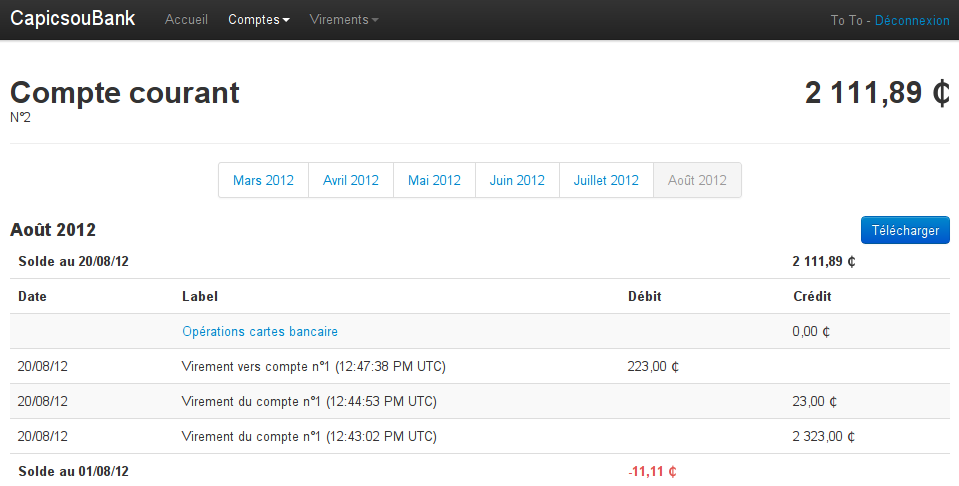
\includegraphics[width=\linewidth]{images/capicsoubank.pdf}
	\caption{Résumé du compte pour le mois d'août}
\end{figure}

L'application est disponible à l'adresse : \url{http://capicsoubank.j.layershift.co.uk}. Pour se connecter, on peut utiliser le compte avec le nom d'utilisateur \verb+toto+ et le mot de passe \verb+toto+.\\

Cette application nous aura permis de terminer notre formation, en nous faisant la main sur les technologies les plus utilisées dans le monde de l'entreprise. Cette application nous a aussi forcé à faire attention à la façon d'implémenter certains aspects d'une application web, notamment à faire attention aux nombres de requêtes par page.\\

Bien que nous n'avions aucun impératif de performance, nous nous sommes restreints au strict nécessaire en terme d'accès base de données pour garantir un bon fonctionnement, même avec une charge sur le serveur.\\

Enfin, l'utilisation des méthodes Agiles nous a permis de développer rapidement sans avoir le réflexe de tout prévoir avant de véritablement implémenter les fonctionnalités. Avec les méthodes Agiles et toutes les méthodes fonctionnant en itération, il ne faut pas développer plus que nécessaire pour la fonctionnalité en cours. L'avantage est de ne pas avoir de code qui sera peut être utilisé plus tard et qui, en réalité, deviendra très certainement du code mort.
